\documentclass[border=10pt]{standalone}

\usepackage{verbatim}


% my addons
\usepackage{graphicx}
%img path
\graphicspath{ {/home/propeller/Downloads/} }
%end of my addons


\usepackage[utf8]{inputenc}
\usepackage{tikz}
\usetikzlibrary{mindmap,shadows}
\usepackage[hidelinks,pdfencoding=auto]{hyperref}

% Information boxes
\newcommand*{\info}[4][16.3]{%
  \node [ annotation, #3, scale=0.65, text width = #1em,
          inner sep = 2mm ] at (#2) {%
  \list{$\bullet$}{\topsep=0pt\itemsep=0pt\parsep=0pt
    \parskip=0pt\labelwidth=8pt\leftmargin=8pt
    \itemindent=0pt\labelsep=2pt}%
    #4
  \endlist
  };
}


%Extra color defined 
\definecolor{tempGrn}{RGB}{0,153,153}
\definecolor{tempBlock}{RGB}{204,0,102}
\definecolor{tempSec}{RGB}{212,170,19}
%end of extra color

\begin{document}
\begin{tikzpicture}[ every annotation/.style = {draw,
                     fill = white, font = \Large}]
  \path[mindmap,concept color=black!40,text=white,
    every node/.style={concept,circular drop shadow},
    root/.style    = {concept color=black!70,
      font=\large\bfseries,text width=10em},
    level 1 concept/.append style={font=\Large\bfseries,
      sibling angle=45,text width=7.7em,
    level distance=25em,inner sep=0pt},
    level 2 concept/.append style={font=\bfseries,level distance=10em},
    level 3 concept/.append style={font=\bfseries,level distance=50em},
    level 4 concept/.append style={font=\bfseries, sibling angle=65,level distance=50em}
  ]
  node[root] {\Huge Bitcoin} [clockwise from=0]
    child[concept color=blue!60] {
      node (bitCore){{Bitcoin Core}} [clockwise from=90]
    }
    child[concept color=blue, level distance=60em] {
      node[concept, text width = 10em] {{Keys and Addresses (\it e.g. Digital signature, Digital fingerprints)}}
        [clockwise from=50]
      child[ level distance=20em] { node[concept, text width = 10em] (cc)
        {{Cryptography and Cryptocurrency}} }
      child [ level distance=15em]{ node[concept] (pk)
        {{Private key}} }
      child [ level distance=15em]{ node[concept] (publicKeys)
        {{Public keys} }
        % third child
        [clockwise from=340]
        child [level distance = 15em]{node[concept, text width = 10em](ellipticCurve) {{Elliptic curve cryptography}} }
        %end of third child
        }  
      child [ level distance=15em]{ node[concept, text width = 7em] (bitcoinAddress)
        {{Bitcoin Addresses (\textbf{\textit{SHA256, RIPEMD160}})} }}    
    }
    child[concept color=green!40!black, level distance =55em] {
      node[concept](wallets) {{Wallets}}
        [clockwise from=260]
      child { node[concept, text width=9em] (nondet)
        {{Nondeterministic wallet}} }
      child { node[concept, text width=7em] (det)
        {{Deterministic wallet}}
       [clockwise from=210]
        child [level distance = 35em]{node[concept, text width = 10em]{{HD wallet}} 
        [clockwise from=260]
        child [level distance = 20em]{node[concept, text width = 10em](hd) {{HD wallet from the seed }}}
        child [level distance = 20em]{node[concept, text width = 10em](ms) {{Mnemonic to seed}}}
         child [level distance = 20em]{node[concept, text width = 10em](gm) {{Generating mnemonic}}}
                }        
         }
    }
    child[concept color=tempGrn] {
      node[concept,text width =10em]  {{Transactions}}
      [clockwise from=340]
      child { node[concept, text width=9em] (ds)
        {{Digital Signatures (ECDSA)}} }
      child { node[concept, text width=7em](tFees) 
        {{Transaction fees}}}
        child { node[concept, text width=7em](tIn)
        {{Transaction inputs}}}
        child { node[concept, text width=7em] (tOut)
        {{Transaction outputs}}}  
        child { node[concept, text width=7em] (utxo)
        {{UTXO}}}     
    }   
    child[concept color=red!60!black, level distance= 60em] {
      node[concept] {{Bitcoin Network}}
        [counterclockwise from=100]
      child { node[concept,text width = 9em] (pp)
        {{Peer-to-Peer}}}
      child  [level distance = 20em]{ node[concept] 
        {{Node types}} 
        [clockwise from=260]
        child [level distance = 15em]{node[concept, text width = 5em]      {{Reference Client}} }
          child [level distance = 15em]{node[concept, text width = 7em]      {{Full Block Chain Node}} }
            child [level distance = 15em]{node[concept, text width = 5em]      {{Solo Miner}} }
              child [level distance = 15em]{node[concept, text width = 9em]      {{Lightweight(SPV) wallet}} }
                child [level distance = 15em]{node[concept, text width = 5em]      {{Pool Protocol Servers}} }
                  child [level distance = 15em]{node[concept, text width = 5em]      {{Mining Nodes}} }
                   child [level distance = 15em]{node[concept, text width = 9em]      {{Lightweight(SPV) Stratum wallet}} }
        }
      child { node[concept,text width = 7em] (nd)
        {{Network discovery}} }
    }
    child[concept color=tempBlock,level distance= 60em] {
      node[concept] (bc)
        {{Blockchain}}
        [clockwise from=200]
        child { node[concept](mt) {{Merkle Tree}}}
        child { node[concept](gb) {{Genesis Block}}}
        child { node[concept] (bh){{Block Header}}}
        }
    child[concept color=yellow!60!black, level distance=50em] {
      node[concept] (Blogs) {Consensus and Mining} [clockwise from=120]
      child { node[concept, text width=8em](mining) {{Mining}}}    
      child { node[concept,text width=8em] (dc){{Decentralized Consensus}} }  
    }
    child[concept color=tempSec, level distance = 50em] {
      node[concept] (Blogs) {Bitcoin Security} [clockwise from=50]
      child { node[concept, text width=8em](bprac) {{Best Practices}} }
      child { node[concept, text width= 8em] (sp)
        {{Security Principle}} }
    };
    \info[30]{bitCore.north east}{above,anchor=west,xshift=1em}{%
      \item Bitcoin core keeps a \textbf{\textit{full copy}} of the blockchain by default, with \textbf{\textit{every transaction}} that has ever occureed on the bitcoin network since its inception in 2009.
      \vspace{1em}
      \item By default, Bitcoin Core builds a database containing \textbf{\textit{only}} the transactions related to the user's wallet.
      \vspace{1em}
      \item Common reasons behind running a Bitcoin Core node :
\begin{itemize}
\item To \textbf{\textit{develop}} bitcoin software.
\item To \textbf{\textit{validate}} transactions according to bitcoin's consensus rules.
\item To \textbf{\textit{ support}} bitcoin, running a node makes the network more robust.
\item To avoid relying on third parties to process or validate transactions.
\end{itemize}      
    }
    
    % bitcoin network
    \info[20]{pp.north west}{above,anchor=south, xshift=3em}{%
      \item The network nodes \textbf{\textit{interconnect}} in a mesh network with a \textbf{\textit{flat}} topology.
      \vspace{1em}
      \item There is no \textbf{\textit{server}}, no \textbf{\textit{centralized}} service, and no \textbf{\textit{hierarchy}}
      within the network.
      \vspace{1em}
      \item The term \textbf{\textit{bitcoin network}} refers to the collection of nodes running the bitcoin \textbf{\textit{P2P protocol}}.    
    }
     \info[20]{nd.south west}{below,anchor=north}{%
      \item A new node must discover other bitcoin nodes on the network in order to participate.
      \vspace{1em}
      \item The \textbf{\textit{geographic}} location of other nodes is \textbf{\textit{irrelevant}}; the bitcoin network topology is not geographically defined.
    }
    %end of bitcoin network
    \info[20]{nondet.south}{below,anchor=north,xshift=5em}{%
      \item Each Key is \textbf{\textit{independently}} generated from a \textbf{\textit{random number.}} Also known as, \textbf{\textit{JBOK}} wallet from the phrase \textbf{\textit{Just a Bunch of Keys.}}
      \vspace{1em}
      \item Cumbersome to back up and use all these keys.
      \vspace{1em}
      \item Discouraged for anything  other than simple tests.
    }
    
    \info[23]{wallets.south}{above, anchor=west, yshift=5em,xshift=4em}{%
      \item The word \textbf{\textit{wallet}} refers to a data structure, that is used to \textbf{\textit{store and manage}} user's keys.
      \vspace{1em}
      \item A bitcoing wallet is a \textbf{\textit{keychain}}. It conatins keys.
      \vspace{1em}
      \item \textbf{\textit{Misconception:}} Bitcoin wallet contains bitcoins $\rightarrow$ \textbf{\textit{not TRUE}}.
      \vspace{1em}
      \item Two primery types of wallets, distinguished by whether the keys are related to each other or not. \textbf{\textit{e.g. Nondetermnistic wallet}}, 
      \textbf{\textit{Deterministic wallet}}.
    }
    \info[20]{det.west}{anchor=east, yshift=-15em}{%
      \item All the keys are generated from a \textbf{\textit{single master key,}} known as \textbf{\textit{seed.}}
      \vspace{1em}
      \item \textbf{\textit{Heirarchical deterministic}} or \textbf{\textit{HD}} wallet has a tree like data structure, one of the many \textbf{\textit{key derivation}} methods used in deterministic wallets.\\
      \vspace{1em}
      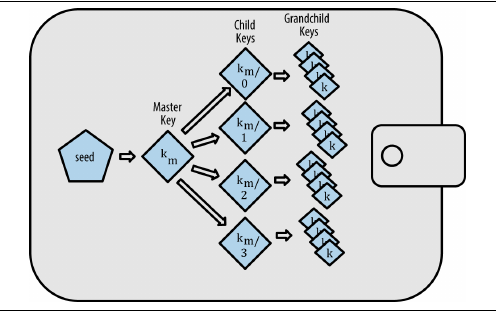
\includegraphics[scale=.45]{hdWallet}
      \item A single backup at creation time is sufficient.
      \vspace{1em}
      \item Allows easy migration of all the user's keys between different wallet implementations.
       \vspace{1em}
       \item The most advanced wallets is the HD wallet defined by the \textbf{\textit{BIP-32}} standard.
       \vspace{1em}
       \item \textbf{\textit{Two}} major advantages using \textbf{\textit{HD wallets}} are: \textbf{\textit{Branches of keys}} can be organized accroding to tasks and functionality. User can create \textbf{\textit{public keys}} without having access to the corresponding private keys.
    }
    \info[30]{pk.south east}{above,anchor=north west}{%
      \item Simply a number, same as " Picking up a number between $1$ and $2^{256}$ "
      \vspace{1em}
      \item More precisely number between $1$ and $n-1$, $n = 1.148 \times 10^{77} $, little less than $2^{256}$,  defined as the order of \textit{elliptic curve} used in bitcoin.
    }
    
    
    \info[22]{bitcoinAddress.south}{below,anchor=north,xshift=-3em}{%
      \item A \textbf{ bitcoin address} is not the same as public key. Bitcoin addresses are derived from public key using a one-way function.
      \vspace{1em}
      \item $A = RIPEMD160(SHA256(K))$
      \vspace{1em}
      \item Always encoded as \textbf{\textit{Base58}} encoding.
      \vspace{1em}
      \item Address begins with \textbf{\textit{`1'}}.
    }
    
    
    \info[20]{publicKeys.south west}{below,anchor=north,yshift=-1em}{%      
      \item Generated form \textbf{\textit{private keys}} using irreversible \textbf{\textit{elliptic curve}} multiplication, $K = k \times G$, where $\textbf{k}$ is the private key, $\textbf{G}$ is a constant point
called $\textbf{\textit{generator point}}$.
	\vspace{1em}
	 \item It is called $\textbf{\textit{trap door}}$ function : it is easy to do only way and reverse is almost impossible. This $\textbf{\textit{mathematical trick}}$ becomes the basis for unforgeable and secure signature.
	 \vspace{1em}
	 \item Reverse operation is known as \textbf{\textit{ finding the discrete loagrithm}}.
    }
    
    
 
    
    \info[30]{cc.east}{anchor=west,xshift = 0.5em}{%
      \item {\textbf{\textit{Prime}} number exponentiation,\textit{\textbf{elliptic}} curve multipication 
      \vspace{1em}
      \item \color{red}Why?}
      \item[] Practically irreversible
      \vspace{1em}
      \item \textbf{\textit{ Asymmetric}} Cryptography $\rightarrow$ Digital signature (Anyone can verify signature, while only owner with private keys can produce valid signatures) 
    }
    \info[17]{ellipticCurve.south}{anchor=west, xshift=5em}{%
      \item Bitcoin uses \textbf{\textit{secp256k1}}, a type of ellipitic curve, established by \textbf{\textit{NIST}}, defined by \textbf{$y^2$ mod $p = (x^3 +7)$ mod $p$}.
      \vspace{1em}
       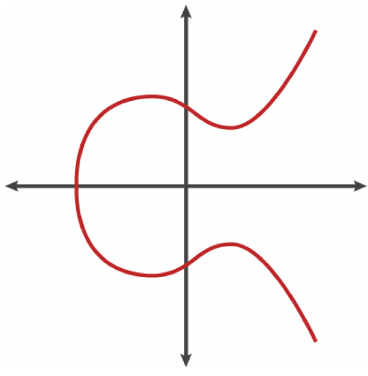
\includegraphics[scale=.35]{ellipticCurve}
       \vspace{1em}
       \item This curve is defined over a \textbf{\textit{fintite field of pime order}} instead of over the \textbf{real numbers},                       
          }
          
          
          %hd wallet info......................
           \info[30]{gm.south}{anchor=east, xshift=-5em,yshift=10em}{%
      \item Mnemonic words are word sequence that represents random number.
      \vspace{1em}
       \item Used as a seed to derive a deterministic wallet.
       \vspace{1em}
       \item \textbf{\textit{Mnemonic}} words are often confused with \textbf{\textit{brainwallets}}.
       \vspace{1em}
       \item The main difference is that a brain wallet consist of words \textbf{\textit{chosen by the user}}, whereas mnemonic words are created \textbf{\textit{randomly by the wallet.}}
       \vspace{1em}
       \item The wallet strats from a source of entropy of \textbf{\textit{128 to 256}} bits, adds a \textbf{\textit{checksum}}, then maps the \textbf{\textit{entropy}} to a \textbf{\textit{wordlist}}.       
       %hd wallet info                    
          }
      \info[30]{ms.south}{anchor=east, xshift=-5em}{%
      \item The \textbf{\textit{key streching}} function \textbf{\textit{PBKDF2}}, is used to generate a longer seed from the mnemonic.
      \vspace{1em}
      \item The key streching function takes two parameters: \textbf{\textit{the mnemonic and a salt}}
      \vspace{1em}
      \item The purpose of a \textbf{\textit{salt}} in a key-streching function is to make it difficult to build a lookup
table enabling a brute-force attack.
       \vspace{1em}
       \item In the \textbf{\textit{BIP-39}} standard, the \textbf{\textit{salt}} allows the introduction of a \textbf{\textit{passphrase}} that serves as an addintional security factor protecting the seed.
       \vspace{1em}
       \item Two important features of passphrase.
       \begin{itemize}   
       \item A second factor:  for protecting mnemonic backups.
       \item \textbf{\textit{Duress wallet}}: to distract an attacker from the \textbf{\textit{real wallet}}. 
       \end{itemize}      
      \vspace{1em}
      \item \textbf{\textit{Passphrase}} also introduces couple of risks:
      \begin{itemize}
      \item If the wallet owner is \textbf{\textit{incapcitated or dead}} and no one know the passphrase, the seed is useless and all the funds stored in the wallet are lost forever.  
         \item If the owner backs up the passphrase in the \textbf{\textit{same place}} as the seed, it defeats pupose of \textbf{\textit{second factor}}.    
\end{itemize}       
}
\info[45]{hd.south}{anchor=north, xshift=-5em}{%
\item \textbf{\textit{HD wallets}} are created a from a single \textit{\textit{root seed}}, which is a \textbf{\textit{128, 356, or 512- bits}} random number.
\vspace{1em}
\item \textbf{\textit{Private child key drivation}} combines:
\begin{itemize}
\item A parent private or public key (ECDSA uncompressed key.)
\item A seed called a \textbf{\textit{chain code}} (256 bits)
\item An \textbf{\textit{index number}} (32 bits)
\end{itemize}
\item[] The \textbf{\textit{public key, chain code, and the index number}} are combined and hashed with the \textbf{\textit{HMAC-SHA512}} algorithm to produce a \textbf{\textit{512-bit}} hash. 
\vspace{1em}
\item[] This 512-bit hash is split into two \textbf{\textit{256-bit}} halves.
\vspace{1em}
\item[] The \textbf{\textit{right-half 256 bits}} of the hash output become the \textbf{\textit{chain code}} for the child. The \textbf{\textit{left-half 256 bits}} of the hash are added to the parent \textbf{\textit{private key}} to produce the child private key. 
\vspace{1em} 
\item \textbf{\textit{Using derived child keys}}:
\item[] A \textbf{\textit{child private key}}, the corresponding \textbf{\textit{public key}}, and the \textbf{\textit{bitcoin address}} are all \textbf{\textit{indstinguishable}} from the keys and addresses created randomly. Once created, they operate exactly as \textbf{\textit{normal}} keys. 
\vspace{1em}
\item \textbf{\textit{Extended Keys}}:
\item[] An extended key consists of a \textbf{\textit{private or public}} key and \textbf{\textit{chain code}}. An extended key can create \textbf{\textit{children}}, generating its own branch in the tree structure. \textbf{\textit{Extended key}} could also be thought of as \textbf{\textit{extensible key}}.
\vspace{1em}
\item \textbf{\textit{Public child key derivation}}:
\item[]  It helps \textbf{\textit{HD wallet}} to derive public keys from pulic parent keys, \textbf{\textit{without}} having the \textbf{\textit{private keys}}. This gives two ways to derive a child public key: either from the \textbf{\textit{child private key}}, or directly from the parent \textbf{\textit{public key}}.
 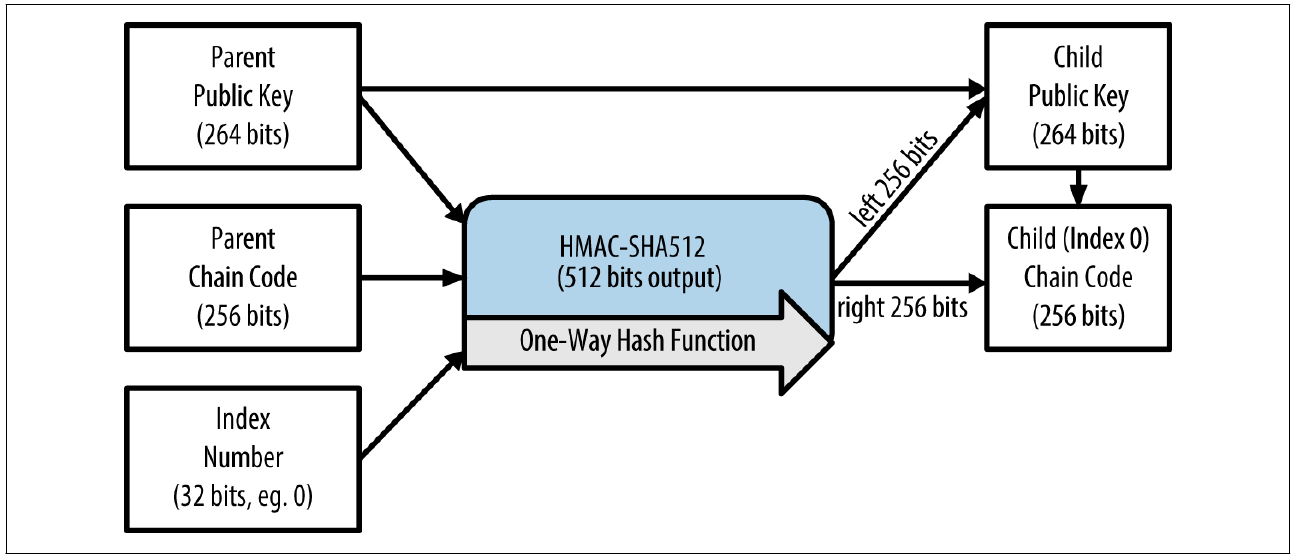
\includegraphics[scale=.45]{eKey}
}
%end of hd wallet info.............................

% transaction info
\info[20]{utxo.north west}{above,anchor=south,xshift=2em}{%
      \item \textbf{\textit{UTXO}} is short form of the  \textbf{\textit{Unspent Transaction Outputs}}.
      \vspace{1em}
      \item The collection of all UTXO is known as the UTXO \textbf{\textit{set}}.
      \vspace{1em}
      \item The UTXO set grows as new UTXO is \textbf{\textit{created}} and shrinks when UTXO is \textbf{\textit{consumed}}.
      \vspace{1em}
      \item Most wallets maintain a database or use a database to store a quick reference set of all the UTXO.
    }
    
    
    \info[20]{tOut.north west}{above,anchor=south,xshift = -6em}{%
      \item Transacton outputs consist of two parts:
      \begin{itemize}
      \item An \textbf{\textit{amount}} of bitcoin. denomintaed in \textbf{\textit{satoshis}}, the smallest bitcoin unit.
      \item A \textbf{\textit{cryptographic}} puzzle that determines the conditions required to spend the output.
      \end{itemize}
    }
    
    \info[30]{tIn.west}{anchor=east, yshift=-5em}{%
      \item The input contains four elements:
      \begin{itemize}
      \item A \textbf{\textit{transaction ID}}, referencing the transaction that contains the UTXO being spent.
      \item An \textbf{\textit{output index}} (vout), identifying which UTXO from that transaction is referenced.
      \item A \textbf{\textit{scriptSig}} which satisfies the conditions placed on the UTXO, unlocking it for spending.
      \item A \textbf{\textit{sequence number}}. 
      \end{itemize}
    }
    
 \info[30]{tFees.south}{anchor=north, xshift=3em}{%
\item \textbf{\textit{Transaction fees}} are collected by the \textbf{\textit{miner}} who mines the block that records the transaction on the \textbf{\textit{blockchain}}.
\vspace{1em}
\item It also serve as a \textbf{\textit{disincentive}} against abuse of the system by imposing a small cost on every transaction.
\item Two types of transaction fees:
\begin{itemize}
\item Static (no longer viable)
\item Dynamic
\end{itemize}
\item Transaction scripts are not \textbf{\textit{Turing complete}}, this ensures no \textbf{\textit{infinite loop}}. 
}
%end transaction info

% blockchain info
\info[20]{bh.north east}{above,anchor=west,xshift=1em}{%
      \item Contains three sets of block metadata:
      \begin{itemize}
      \item Referance to a \textbf{\textit{previous block hash}}.
      \item \textbf{\textit{Difficulty, timestamp, nonce}}.
      \item \textbf{\textit{Merkle tree root}}.      
      \end{itemize}
    }
 \info[30]{mt.south}{anchor=east, xshift=-2em,yshift=5em}{%
      \item Merkle tree is a data sturcture used for efficiently \textbf{\textit{summarizing and verifying}} the \textbf{\textit{integrity}} of large sets of data.                          
          }
          
\info[30]{gb.south}{anchor=east, xshift=-2em,yshift=5em}{%
      \item \textbf{\textit{First block}} and \textbf{\textit{common ancestor}} of all the blocks in the blockchain, created in \textbf{\textit{2009}}.
      \vspace{1em}
      \item A secure root to build a trusted blockchain.                       
          }
          
 \info[23]{bc.south}{above, anchor=west, yshift=-4em,xshift=4em}{%
      \item An \textbf{\textit{ordered}}, \textbf{\textit{back-linked}} list of blocks of transactions.
      \vspace{1em}
      \item The existence of a long chain of bloks makes the blockchain's deep history \textbf{\textit{immutable}}, which is a key feature of bitcoin's security.
      \vspace{1em}
      \item The term \textbf{\textit{height}} refers to the distance from the first block, and \textbf{\textit{top}} or \textit{\textbf{tip}} refers to the most recently added block. 
    }
 % end of blockchain info
 %mining info
  \info[30]{mining.south}{anchor=east, xshift=-2em,yshift=15em}{%
      \item Mining \textbf{\textit{secures}} the bitcoin system and enables the emergence of network-wide \textbf{\textit{consensus}} without a \textbf{\textit{central authority}}.
      \vspace{1em}
      \item Miners validate \textbf{\textit{Proof-of-Work}} by solving a mathematical problem based on \textbf{\textit{cryptographic hash algorithm}}.
      \vspace{1em}
      \item Bitcoin miners receive two types of rewards by mining:
      \begin{itemize}
      \item New coins created with each new block.
      \item Transaction fees.
      \end{itemize}
      \item The maximum amount of newly created bitcoin a miner can add decreases approximately every \textbf{\textit{four years}}.
          }
          \info[30]{dc.north east}{above,anchor=west,xshift=1em}{%
      \item \textbf{\textit{Satoshi Nakamoto's}} main invention is the decentralized mechanism for \textbf{\textit{emergent consensus}}.
      \vspace{1em}
      \item \textbf{\textit{Consensus}} is an emergent artifact of the \textbf{\textit{asynchronous interaction}} of thousands of independent nodes.
      \vspace{1em}
      \item Bitcoin's \textbf{\textit{decentralized consensus}} emerges from the interplay of \textbf{\textit{four processes}}:
      \begin{itemize}
      \item Independent verifiaction of each transaction, by every full node.
      \item Independent aggregation of those transactions into new blocks by mining nodes.
      \item Independent verification of the new blocks by every node.
      \item Independent selection, by every node, of the chain with the most cumulative computation demonstrated through \textbf{\textit{Proof-of-work}}.
\end{itemize}       
    }
 % end of mining info
 % security info
 \info[30]{sp.east}{anchor=south west, yshift=-20em}{%
      \item The core \textbf{\textit{principle}} in bitcoin is \textbf{\textit{decentralization}}.
      \vspace{1em}
      \item Security of the network is based on \textbf{\textit{Proof-of-work}}.
      \vspace{1em}
      \item A bitcoin only a \textbf{\textit{specific value}} to a \textbf{\textit{specific recipent}} and cannot be \textbf{\textit{forged and modified}}.
      \vspace{1em}
      \item Does not reveal any \textbf{\textit{private information}}, such as the identities of the parties.
      \vspace{1em}
      \item \textbf{\textit{Root of trust}} is the \textbf{\textit{decentralized block chain ledger}}.
      \vspace{1em}
      \item The \textbf{\textit{root of trust}} concept ensures that most of the trust is placed within the least complex part of the system, and therfore least vulnerable, parts of the system, while more complex software is layered around it.
    }
     \info[20]{bprac.north west}{above,anchor=south, xshift=3em}{%
      \item \textbf{\textit{Physical Bitcoin Storage}}
      \vspace{1em}
      \item \textbf{\textit{Hardware Wallets}}
      \vspace{1em}
      \item \textbf{\textit{Balancing Risk}}
      \vspace{1em}
      \item \textbf{\textit{Diversifying Risk}}
      \vspace{1em}
      \item \textbf{\textit{Multisig and Governance}}
      \vspace{1em}
      \item \textbf{\textit{Survivability}}          
    }
    %end security info
    
    %extra info
    \info[85]{det.west}{anchor=east, xshift=45em, yshift=-68em}{%
      \item \textbf{{\huge Bitcoin Core Node Architechture:}}
      \vspace{2em}
      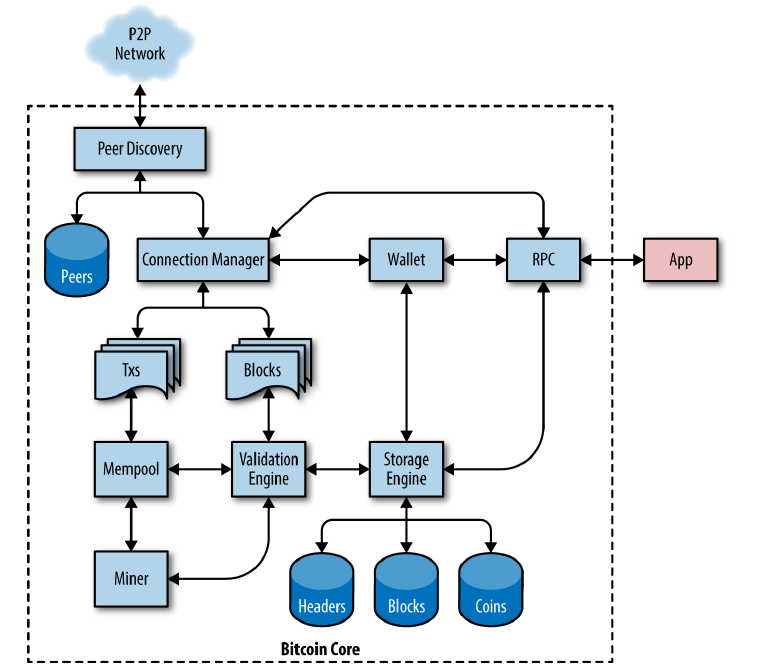
\includegraphics[scale=1.5]{core}
    }
    \info[85]{ellipticCurve.south}{anchor=west, yshift=-60em, xshift=-5em}{%
    \item \textbf{\huge Different Types of Bitcoin Nodes}\\
    \vspace{1em}
       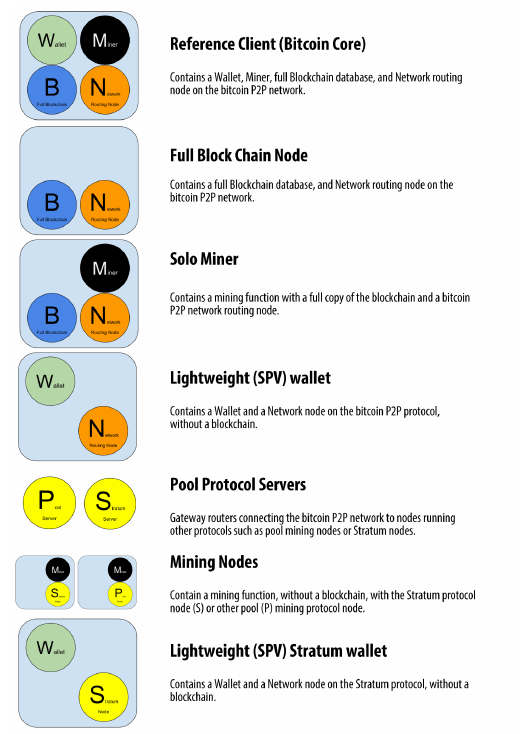
\includegraphics[scale=1.75]{nodes}                      
          }
          \info[50]{dc.north east}{above,anchor=west,xshift=70em, yshift= 10em}{%
      \item \Huge MD. Galib Ahsan
      \vspace{1em}
      \item \Huge ID: 20166062
    }
\end{tikzpicture}
\end{document}

